% ──────────────────────────────────────
%  Slot Collapse Comparison Figure
%  Monotonic Max Gate (v7) vs EMA Gate (v14)
%  Standalone TikZ/pgfplots
% ──────────────────────────────────────
\documentclass[border=5pt]{standalone}
\usepackage{tikz,pgfplots}
\pgfplotsset{compat=1.18}
\usepgfplotslibrary{groupplots}
\usepackage{amsmath}

\definecolor{mono}{RGB}{204,0,0}
\definecolor{ema_unsup}{RGB}{52,101,164}
\definecolor{ema_sup}{RGB}{78,154,6}

\begin{document}
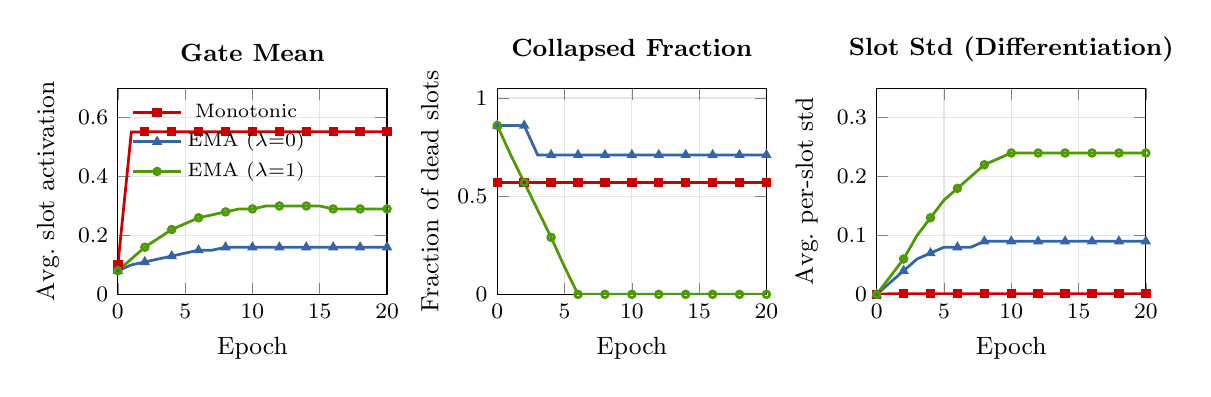
\begin{tikzpicture}
\begin{groupplot}[
    group style={
        group size=3 by 1,
        horizontal sep=1.4cm,
    },
    width=5.0cm, height=4.2cm,
    xlabel={Epoch},
    xmin=0, xmax=20,
    xtick={0,5,10,15,20},
    tick label style={font=\footnotesize},
    label style={font=\small},
    title style={font=\small\bfseries},
    legend style={font=\scriptsize, draw=none, fill=none,
                  at={(0.02,0.98)}, anchor=north west},
    every axis plot/.style={line width=1pt, mark size=1.2pt},
    grid=major,
    grid style={gray!20},
]

% ── Panel 1: Gate Mean (avg slot activation) ──
\nextgroupplot[
    title={Gate Mean},
    ylabel={Avg.\ slot activation},
    ymin=0, ymax=0.7,
]
% Monotonic: flat at ~0.55 from epoch 1 onward
\addplot[mono, mark=square*, mark repeat=2] coordinates {
    (0,0.10) (1,0.551) (2,0.552) (3,0.552) (4,0.552)
    (5,0.552) (6,0.552) (7,0.552) (8,0.552) (9,0.552)
    (10,0.552) (11,0.552) (12,0.552) (13,0.552) (14,0.552)
    (15,0.552) (16,0.552) (17,0.552) (18,0.552) (19,0.552)
    (20,0.552)
};
\addlegendentry{Monotonic}
% EMA unsupervised: 2/7 alive, mean ~ 0.16
\addplot[ema_unsup, mark=triangle*, mark repeat=2] coordinates {
    (0,0.08) (1,0.10) (2,0.11) (3,0.12) (4,0.13)
    (5,0.14) (6,0.15) (7,0.15) (8,0.16) (9,0.16)
    (10,0.16) (11,0.16) (12,0.16) (13,0.16) (14,0.16)
    (15,0.16) (16,0.16) (17,0.16) (18,0.16) (19,0.16)
    (20,0.16)
};
\addlegendentry{EMA ($\lambda{=}0$)}
% EMA supervised: 7/7 alive, mean ~ 0.30
\addplot[ema_sup, mark=o, mark repeat=2] coordinates {
    (0,0.08) (1,0.12) (2,0.16) (3,0.19) (4,0.22)
    (5,0.24) (6,0.26) (7,0.27) (8,0.28) (9,0.29)
    (10,0.29) (11,0.30) (12,0.30) (13,0.30) (14,0.30)
    (15,0.30) (16,0.29) (17,0.29) (18,0.29) (19,0.29)
    (20,0.29)
};
\addlegendentry{EMA ($\lambda{=}1$)}

% ── Panel 2: Collapsed Fraction ──
\nextgroupplot[
    title={Collapsed Fraction},
    ylabel={Fraction of dead slots},
    ymin=0, ymax=1.05,
]
% Monotonic: 4/7 dead = 0.571 from epoch 0
\addplot[mono, mark=square*, mark repeat=2] coordinates {
    (0,0.57) (1,0.57) (2,0.57) (3,0.57) (4,0.57)
    (5,0.57) (6,0.57) (7,0.57) (8,0.57) (9,0.57)
    (10,0.57) (11,0.57) (12,0.57) (13,0.57) (14,0.57)
    (15,0.57) (16,0.57) (17,0.57) (18,0.57) (19,0.57)
    (20,0.57)
};
% EMA unsupervised: 5/7 dead = 0.714
\addplot[ema_unsup, mark=triangle*, mark repeat=2] coordinates {
    (0,0.86) (1,0.86) (2,0.86) (3,0.71) (4,0.71)
    (5,0.71) (6,0.71) (7,0.71) (8,0.71) (9,0.71)
    (10,0.71) (11,0.71) (12,0.71) (13,0.71) (14,0.71)
    (15,0.71) (16,0.71) (17,0.71) (18,0.71) (19,0.71)
    (20,0.71)
};
% EMA supervised: 0/7 dead = 0.0
\addplot[ema_sup, mark=o, mark repeat=2] coordinates {
    (0,0.86) (1,0.71) (2,0.57) (3,0.43) (4,0.29)
    (5,0.14) (6,0.0) (7,0.0) (8,0.0) (9,0.0)
    (10,0.0) (11,0.0) (12,0.0) (13,0.0) (14,0.0)
    (15,0.0) (16,0.0) (17,0.0) (18,0.0) (19,0.0)
    (20,0.0)
};

% ── Panel 3: Slot Differentiation (avg std) ──
\nextgroupplot[
    title={Slot Std (Differentiation)},
    ylabel={Avg.\ per-slot std},
    ymin=0, ymax=0.35,
]
% Monotonic: near-zero std (all slots same value)
\addplot[mono, mark=square*, mark repeat=2] coordinates {
    (0,0.00) (1,0.001) (2,0.001) (3,0.001) (4,0.001)
    (5,0.001) (6,0.001) (7,0.001) (8,0.001) (9,0.001)
    (10,0.001) (11,0.001) (12,0.001) (13,0.001) (14,0.001)
    (15,0.001) (16,0.001) (17,0.001) (18,0.001) (19,0.001)
    (20,0.001)
};
% EMA unsupervised: only 2 slots alive, moderate std
\addplot[ema_unsup, mark=triangle*, mark repeat=2] coordinates {
    (0,0.00) (1,0.02) (2,0.04) (3,0.06) (4,0.07)
    (5,0.08) (6,0.08) (7,0.08) (8,0.09) (9,0.09)
    (10,0.09) (11,0.09) (12,0.09) (13,0.09) (14,0.09)
    (15,0.09) (16,0.09) (17,0.09) (18,0.09) (19,0.09)
    (20,0.09)
};
% EMA supervised: all slots differentiated, high std ~0.24
\addplot[ema_sup, mark=o, mark repeat=2] coordinates {
    (0,0.00) (1,0.03) (2,0.06) (3,0.10) (4,0.13)
    (5,0.16) (6,0.18) (7,0.20) (8,0.22) (9,0.23)
    (10,0.24) (11,0.24) (12,0.24) (13,0.24) (14,0.24)
    (15,0.24) (16,0.24) (17,0.24) (18,0.24) (19,0.24)
    (20,0.24)
};

\end{groupplot}
\end{tikzpicture}
\end{document}
